
\subsection{Cleanup}


\begin{figure}[ht]
	\begin{minipage}[t][13cm][t]{0.5\textwidth}
		At the end of each turn, the players set up the board for the next turn.
		\begin{itemize}
			\item \textbf{Boons \& Banes} - If relevant, apply poison damage and remove any single-turn boon or bane. \textit{(See "Boons \& Banes", page \pageref{Section_BoonsBanes})} \\
			\item \textbf{Rotate} - Move your \textbf{leftmost} (sideways) enemy to the next player clockwise. This happens \textbf{simultaneously}. You cannot give away an enemy given to you this way\\
			\item \textbf{Backlined} - If your life is 0, give all your remaining enemies to your left. Without an opponent to fight, all of your \textbf{remaining enemies rotate} to the left.
			Enemies will never move to a backlined player, instead immediately rotating to the next fighting player
			\begin{tcolorbox}[colframe=blue, colback=white]
				Reminder - This can result into floods of enemies tearing through the rest of the party, so be careful!
			\end{tcolorbox}
			\item \textbf{Wheel} - Rotate the inner part of the Wheel of Elements clockwise. This changes the cubes on the outer side of the wheel to another element, and it changes the enemies attack pattern\\
			\item \textbf{Retain} - You keep all cards you did not play in your hand\\
			
		\end{itemize}
		
	\end{minipage}	
	\begin{minipage}[t][11cm][t]{0.5\textwidth}
		\centering
		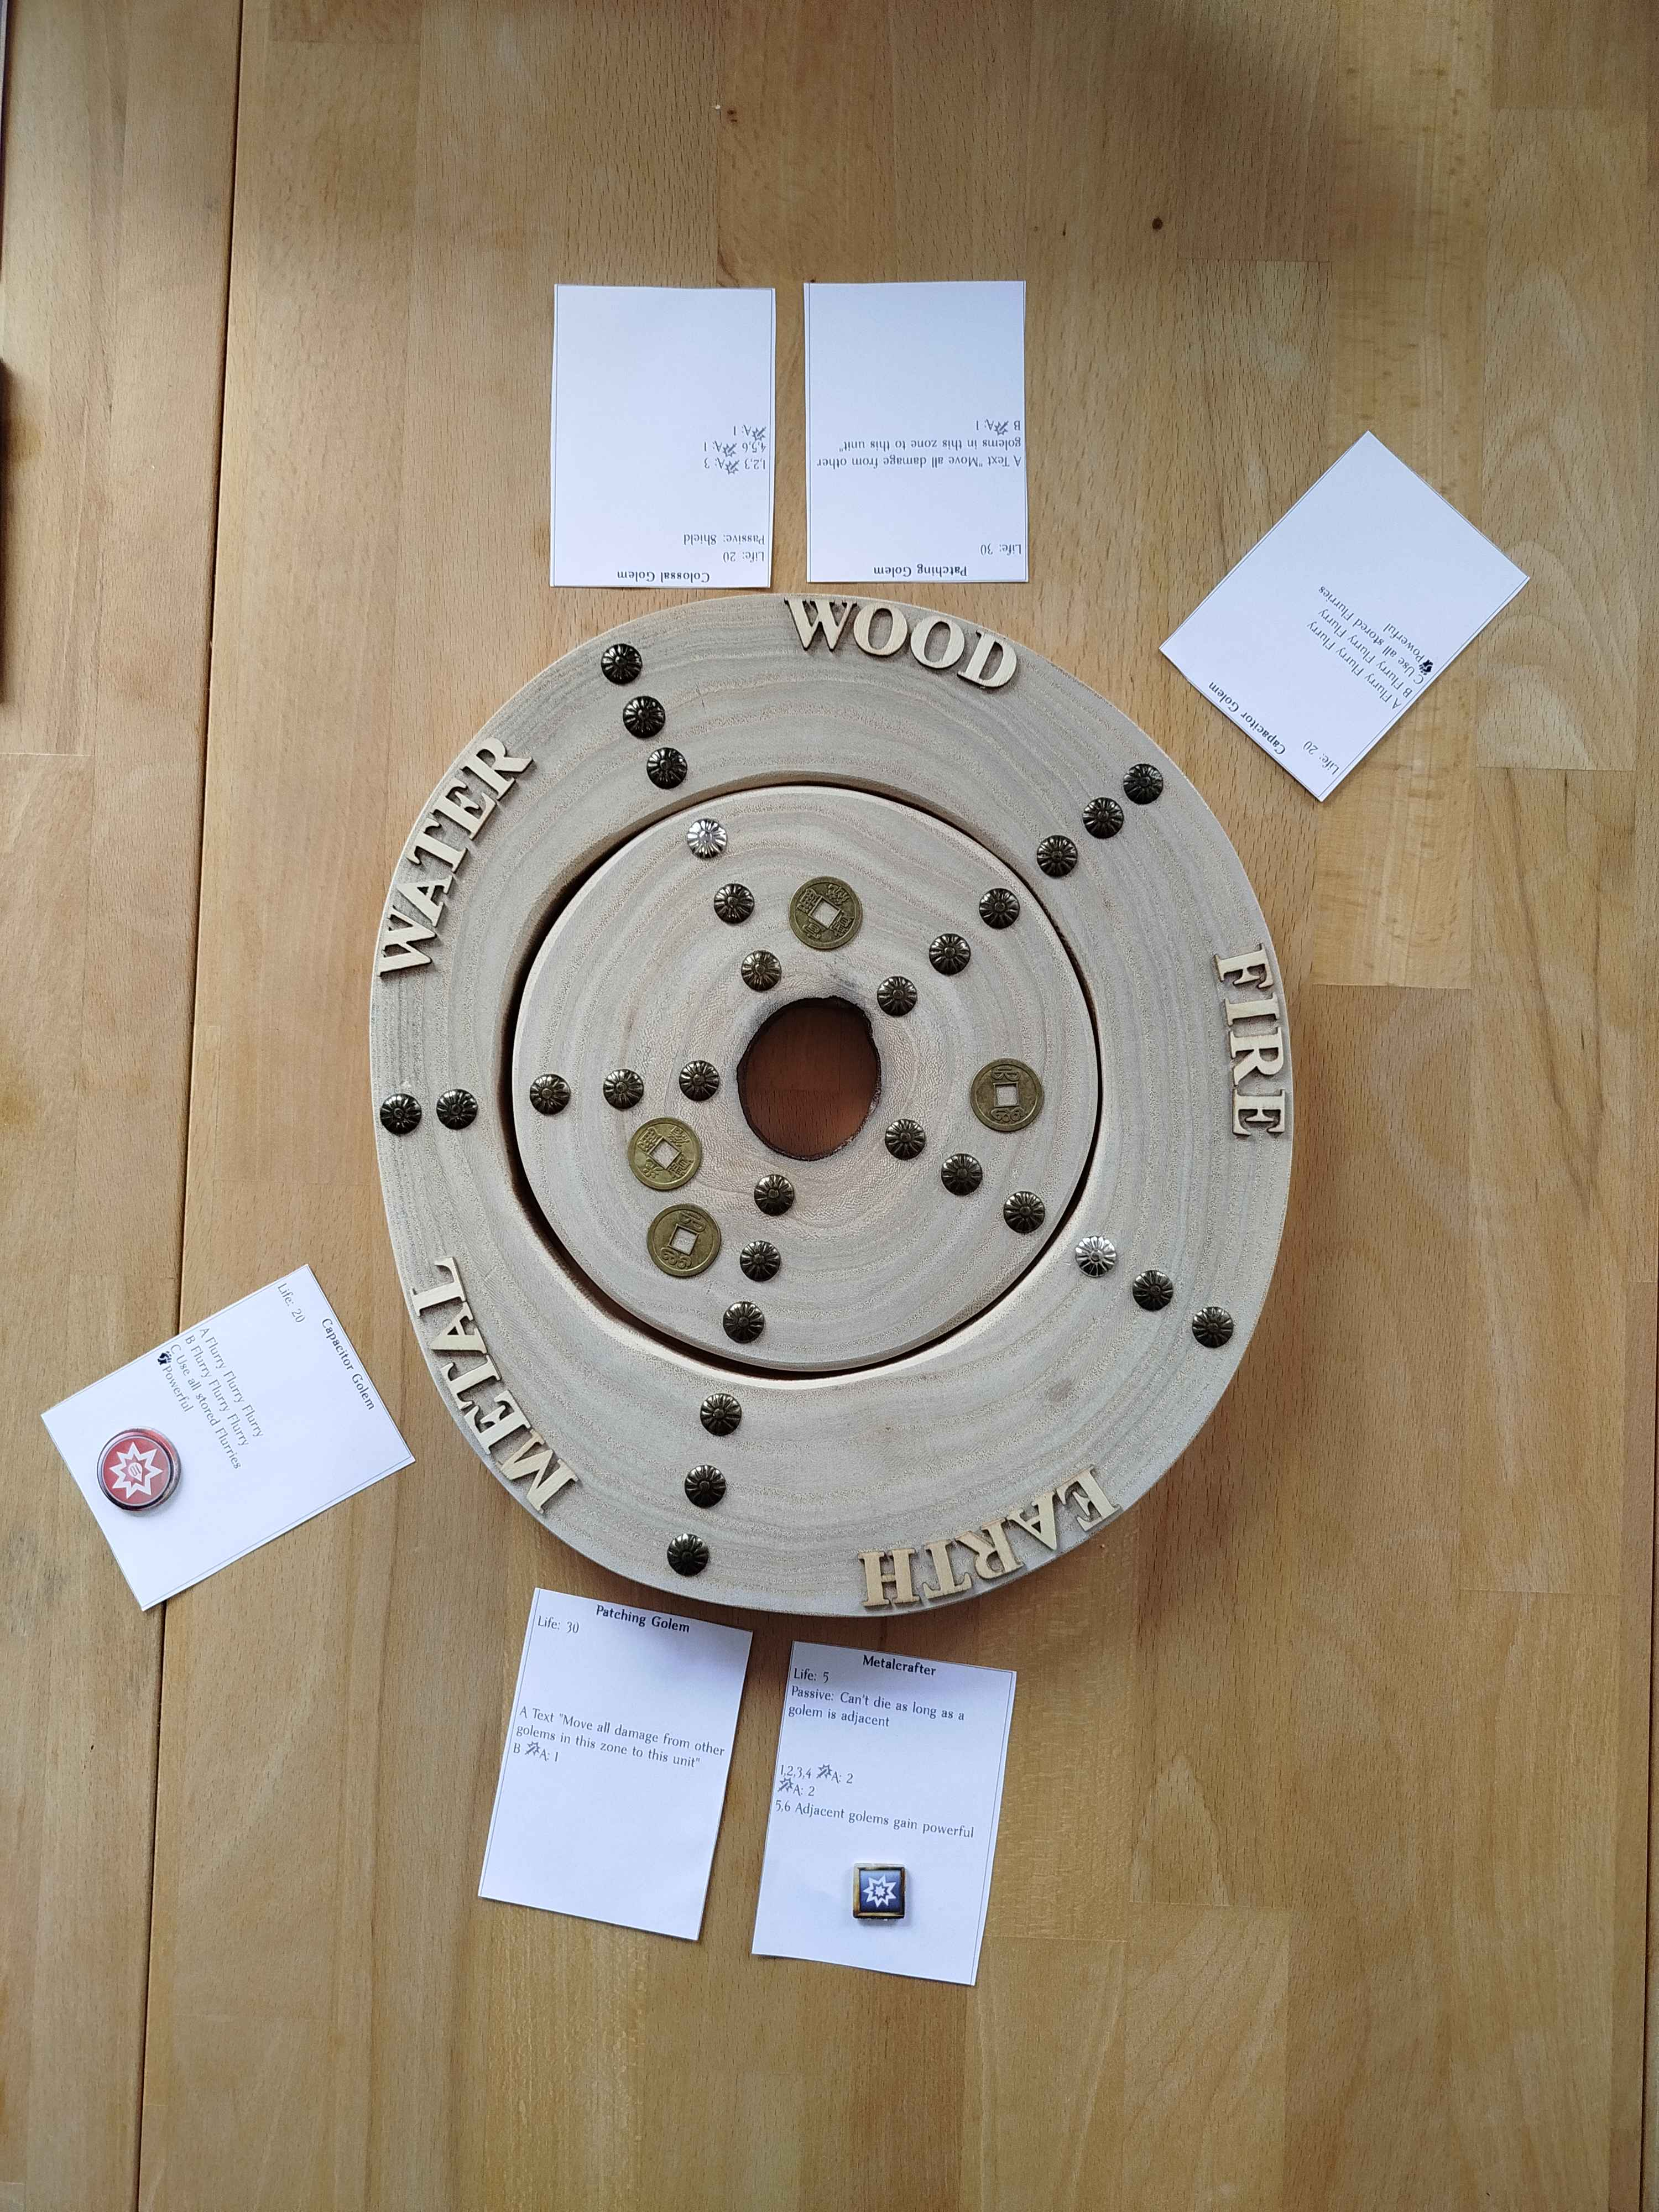
\includegraphics[width=0.9\linewidth, valign=t]{../ExplanationPics/RotaExample.jpg}
	\end{minipage}
\end{figure}
%\begin{tcolorbox}[colframe=black, colback=white]
%	Turning the enemies sideways is only used as indicator, nothing more. %They also have a little nap during rotation.
%\end{tcolorbox}



